\columnbreak
\section{Koordinatensysteme}
\subsection{2D Koordinatensysteme}
Neben den Kartesischen Koordinatensystemen kommen in zweidimensionalen Räumen auch Polare Koordinatensysteme zum Einsatz.
Die beiden Systeme können mit Hilfe der Trigonometrie in einander überführt werden.

\subsubsection{Umrechnung Kartesisch $\leftrightarrow$ Polar}
\begin{minipage}{0.29\linewidth}
    \myul{Polar zu Kartesisch}
    \[
    \begin{pmatrix}
        x \\
        y
    \end{pmatrix}
    =
    \begin{pmatrix}
        r \cdot \cos{\varphi}\\
        r \cdot \sin{\varphi}
    \end{pmatrix}
    \]
\end{minipage}
\hfill
\begin{minipage}{0.29\linewidth}
    \myul{Kartesisch zu Polar}
    \[
    \begin{pmatrix}
        r \\
        \varphi
    \end{pmatrix}
    =
    \begin{pmatrix}
        \sqrt{x^2+y^2}\\
        \tan^{-1}{\frac{y}{x}}
    \end{pmatrix}
    \]
\end{minipage}
\hfill
\begin{minipage}{0.29\linewidth}
    \begin{center}
        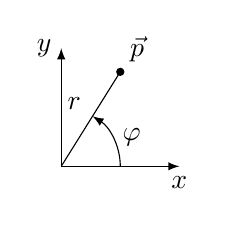
\begin{tikzpicture} [scale = 1.5]
            % Kartesische Achsen
            \draw[-{latex}] (0, 0) -- (1, 0) node [below] {$x$} ;
            \draw[-{latex}] (0, 0) -- (0, 1) node [left]  {$y$} ;

            % Punkt p
            \fill (0.5, 0.8) circle (1pt) node [anchor=south west] {$\vec{p}$};

            % Länge r
            \draw (0, 0) -- (0.5, 0.8) node [midway, above left] {$r$};
            % Winkel phi
            \draw [-{latex}] (0.5, 0) arc (0:58:0.5) node [midway, right] {$\varphi$};
        \end{tikzpicture}
    \end{center}
\end{minipage}

Dabei ist zu beachten, dass $\tan^{-1}$ nur werte von $-\frac{\pi}{2}$ bis $\frac{\pi}{2}$ liefert, für $\varphi$ jedoch $\varphi \in [0, \pi]$ gelten soll. 
$\varphi$ wird also, je nach dem in welchem Quadranten sich $\vec{p}$ befindet, nach folgendem Schema berechnet:
\begin{center}
    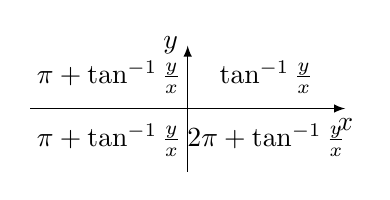
\begin{tikzpicture}
        % Achsen 
        \draw [-{latex}] (-2, 0) -- (2, 0) node [below] {$x$};
        \draw [-{latex}] (0, -0.8) -- (0, 0.8) node [left] {$y$};
        % Formeln
        \node at ( 1,  0.4) {$       \tan^{-1}\frac{y}{x}$};
        \node at ( 1, -0.4) {$2\pi + \tan^{-1}\frac{y}{x}$};
        \node at (-1, -0.4) {$\pi  + \tan^{-1}\frac{y}{x}$};
        \node at (-1,  0.4) {$\pi  + \tan^{-1}\frac{y}{x}$};
    \end{tikzpicture}
\end{center}

Um eine ganzes Integral vom einen Koordinatensystem ins andere zu überführen, muss zum einen die Funktion $ f(x, y) $ zu $ f(r, \varphi) $ (oder umgekehrt) umgeschrieben, sowie die differentiale angepasst werden.
Hier dafür einige gängige Elemente:

\begin{tabular}{l c c}
                         & \bf{Kartesisch}                   & \bf{Polar}                                                       \\
    \bf{x-Achsenelement} & $\diff x$                         & $\diff x = \cos \varphi \diff r - r \sin \varphi \diff \varphi$  \\
    \bf{y-Achsenelement} & $\diff y$                         & $\diff x = \sin \varphi \diff r + r \cos \varphi \diff \varphi$  \\
    \bf{Linienelement  } & $\diff s^2 = \diff x^2 \diff y^2$ & $\diff s^2 = \diff r^2 + r^2 \diff \varphi^2$                    \\
    \bf{Flächenelement } & $\diff A = \diff x \diff y$       & $\diff A = r \diff r \diff \varphi$                              \\
\end{tabular}


\subsection{3D Koordinatensysteme}
\resizebox{\linewidth}{!}{
    \begin{tabular}{c c c}
        \myul{\textbf{Kartesisch}} & \myul{\textbf{Zylindrisch}} & \myul{\textbf{Sphärisch}} \\
        
        \tdplotsetmaincoords{70}{110}
        \begin{tikzpicture}[baseline=(current bounding box.north), tdplot_main_coords, scale=2]
            % Koordinatensystem
            \draw [-{latex}] (0, 0, 0) -- (1, 0, 0) node [below left] {$x$};
            \draw [-{latex}] (0, 0, 0) -- (0, 1, 0) node [right]      {$y$};
            \draw [-{latex}] (0, 0, 0) -- (0, 0, 1) node [right]      {$z$};
            % Punkt bei (0.75,0.75,0.75)
            \fill (0.75, 0.75, 0.75) circle (1pt) node [above right] {$P(x, y, z)$};
            % Koordinatenkomponenten
            \draw [dashed] (0, 0.75, 0)    -- (0.75, 0.75, 0)    node [midway, below right] {$x$};
            \draw [dashed] (0.75, 0, 0)    -- (0.75, 0.75, 0)    node [midway, below left]  {$y$};
            \draw [dashed] (0.75, 0.75, 0) -- (0.75, 0.75, 0.75) node [midway, right]       {$z$};
        \end{tikzpicture} &

        \tdplotsetmaincoords{70}{110}
        \begin{tikzpicture}[baseline=(current bounding box.north), tdplot_main_coords, scale=2]
            % Koordinatensystem
            \draw [-{latex}] (0, 0, 0) -- (1, 0, 0) node [below left] {$x$};
            \draw [-{latex}] (0, 0, 0) -- (0, 1, 0) node [right]      {$y$};
            \draw [-{latex}] (0, 0, 0) -- (0, 0, 1) node [right]      {$z$};
            % Punkt bei (0.75,0.75,0.75)
            \fill (0.75, 0.75, 0.75) circle (1pt) node [above right] {$P(r_{\rm z}, \varphi, z)$};
            % Koordinatenkomponenten
            \draw [dashed] (0,0,0)         --  (0.75, 0.75, 0)    node [midway, above right, inner sep=0pt] {$r_{\rm z}$};
            \draw [-{latex}]     (0.5,0,0)       arc (0:45:0.5)         node [midway, below]       {$\varphi$};
            \draw [dashed] (0.75, 0.75, 0) --  (0.75, 0.75, 0.75) node [midway, right]       {$z$};
        \end{tikzpicture} &

        \tdplotsetmaincoords{70}{110}
        \begin{tikzpicture}[baseline=(current bounding box.north), tdplot_main_coords, scale=2]
            % Koordinatensystem
            \draw [-{latex}] (0, 0, 0) -- (1, 0, 0) node [below left] {$x$};
            \draw [-{latex}] (0, 0, 0) -- (0, 1, 0) node [right]      {$y$};
            \draw [-{latex}] (0, 0, 0) -- (0, 0, 1) node [right]      {$z$};
            % Punkt bei (0.75,0.75,0.75)
            \fill (0.75, 0.75, 0.75) circle (1pt) node [above right] {$P(r_{\rm s}, \theta, \phi)$};
            % Koordinatenkomponenten
            \draw [dotted] (0,0,0) -- (0.75, 0.75, 0) -- (0.75, 0.75, 0.75);
            \draw [-{latex}]     (0.5,0,0) arc (0:45:0.5)         node [midway, below]       {$\phi$};
            \draw [dashed] (0, 0, 0) --  (0.75, 0.75, 0.75) node [midway, below right] {$r_{\rm s}$};
            \tdplotsetthetaplanecoords {90}
            \tdplotdrawarc [tdplot_rotated_coords, -{latex}] {(0, 0, 0)} {0.5} {0} {45} {anchor=south} {$\theta$}
        \end{tikzpicture} \\

        $ 
        \begin{pmatrix}
            x \\ y \\ z
        \end{pmatrix} 
        =
        \begin{pmatrix}
            r \cos \varphi \\ r \sin \varphi \\ z
        \end{pmatrix}
        =
        \begin{pmatrix}
            r \sin \theta \cos \phi \\ r \sin \theta \sin \phi \\ r \cos \theta
        \end{pmatrix}
        $ &
        $ 
        \begin{pmatrix}
            r_{\rm z} \\ \varphi \\ z
        \end{pmatrix} 
        =
        \begin{pmatrix}
            \sqrt{x^2 + y^2} \\ \tan^{-1}\frac{y}{x} \\ z
        \end{pmatrix}
        =
        \begin{pmatrix}
            r_{\rm s} \sin \theta \\ \phi \\ r_{\rm s} \cos \theta
        \end{pmatrix}
        $ &
        $ 
        \begin{pmatrix}
            r_{\rm s} \\ \theta \\ \phi
        \end{pmatrix} 
        =
        \begin{pmatrix}
            \sqrt{x^2+y^2+z^2} \\ \cos^{-1} \frac{z}{\sqrt{x^2+y^2+z^2}} \\ \sgn(y) \cos^{-1} \frac{x}{\sqrt{x^2+y^2}}
        \end{pmatrix}
        =
        \begin{pmatrix}
            \sqrt{r_{\rm z}^2+z^2} \\ \tan^{-1}\frac{r_{\rm z}}{z} \\ \varphi
        \end{pmatrix}
        $ \\
    \end{tabular}
}
\smallskip
\subsubsection{Umrechnen zwischen Koordinatensystemen}
Beim Umrechnen zwischen den Koordinatensystemen gelten im Grunde genommen die obigen Formeln. 
Dabei muss jedoch in einigen Fällen auf die Wertebereiche von den trigonometrischen Funktionen rücksicht genommen werden.

\myul{\textbf{Zylindrisch $\rightarrow$ Kartesisch:}}\\
\myul{\textbf{Sphärisch $\rightarrow$ Kartesisch:}}\\
Keine weiteren Berücksichtigungen nötig, die Berechnung erfolgt nach der Formel oben.
\medskip

\myul{\textbf{Kartesisch $\rightarrow$ Zylindrisch:}}\\
\begin{minipage}{0.49\linewidth}
    Der Parameter $\phi$ wird analog zum zweidimensionalen Fall, je nach dem in welchem Quadranten sich $P$ befindet, nach dem Schema rechts berechnet.
\end{minipage}
\hfill
\begin{minipage}{0.49\linewidth}
    \begin{center}
        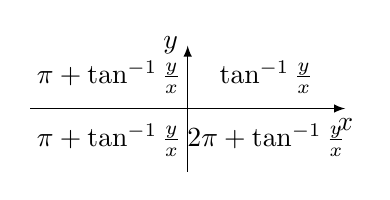
\begin{tikzpicture}
            % Achsen 
            \draw [-{latex}] (-2, 0) -- (2, 0) node [below] {$x$};
            \draw [-{latex}] (0, -0.8) -- (0, 0.8) node [left] {$y$};
            % Formeln
            \node at ( 1,  0.4) {$       \tan^{-1}\frac{y}{x}$};
            \node at ( 1, -0.4) {$2\pi + \tan^{-1}\frac{y}{x}$};
            \node at (-1, -0.4) {$ \pi + \tan^{-1}\frac{y}{x}$};
            \node at (-1,  0.4) {$ \pi + \tan^{-1}\frac{y}{x}$};
        \end{tikzpicture}
    \end{center}
\end{minipage}
\medskip

\myul{\textbf{Sphärisch $\rightarrow$ Zylindrisch:}}\\
\myul{\textbf{Kartesisch $\rightarrow$ Sphärisch:}}\\
Keine weiteren Berücksichtigungen nötig, die Berechnung erfolgt nach der Formel oben.
\medskip

\myul{\textbf{Zylindrisch $\rightarrow$ Sphärisch:}}\\
\begin{minipage}{0.49\linewidth}
    Auch hier macht der $\tan^{-1}$ Probleme, da er Werte von $-\frac{\pi}{2}$ bis $\frac{\pi}{2}$ liefert, für $\theta$ jedoch $\theta \in [0, \pi]$ gelten soll.
    Je nach dem, ob $P$ sich oberhalb oder unterhalb der $xy$-Ebene befindet, wird $\theta$ wie rechts berechnet.
\end{minipage}
\hfill
\begin{minipage}{0.49\linewidth}
    \begin{center}
        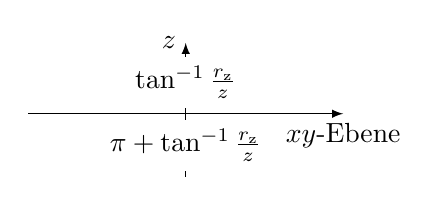
\begin{tikzpicture}
            % Achsen 
            \draw [-{latex}] (-2,  0)   -- (2, 0) node [below] {$xy$-Ebene};
            \draw [-{latex}] ( 0, -0.8) -- (0,.9) node [left]  {$z$};
            % Formeln
            \node [fill=white] at (0,  0.4) {$\tan^{-1}\frac{r_{\rm z}}{z}$};
            \node [fill=white] at (0, -0.4) {$\pi + \tan^{-1}\frac{r_{\rm z}}{z}$};
        \end{tikzpicture}
    \end{center}
\end{minipage}

